\section{Introduction}
\label{sec:intro}

\begin{figure}[t]
\centering
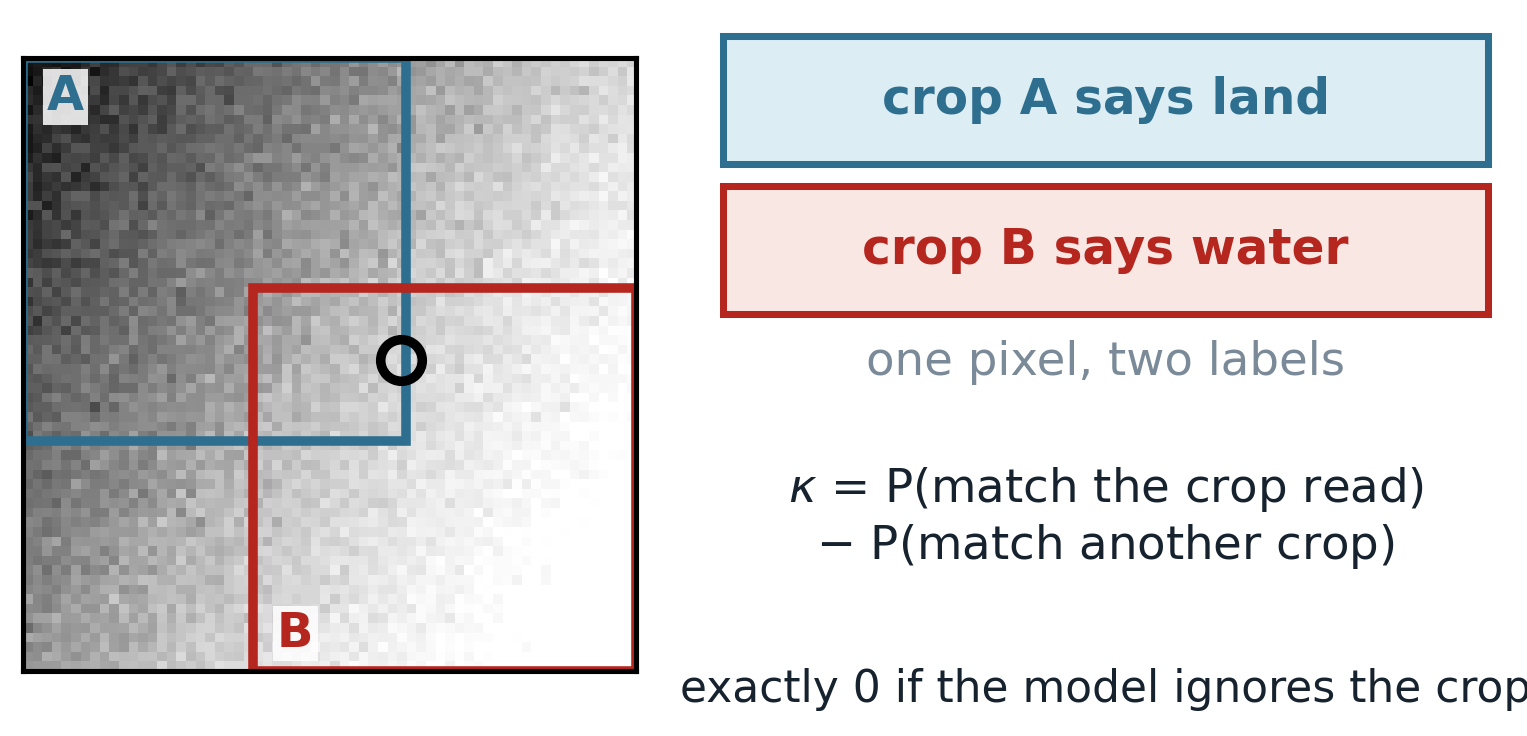
\includegraphics[width=\linewidth]{figures/fig0_mechanism.png}
\caption{The failure this paper measures. A labeller run inside each crop computes a
different threshold in each, here $-21.5$ and $-15.5$\,dB, so a pixel between them
comes out water in one window and land in the other.}
\label{fig:mechanism}
\end{figure}

Auto-labelling made large segmentation benchmarks possible. It also made some of
them circular, because the label can depend on which crop the model reads a pixel
in (\cref{fig:mechanism}). We are not aware of a diagnostic tailored to this
failure with an algebraically fixed reference value. Partial-input baselines answer the neighbouring
question~\cite{goyal2017making, jabri2016revisiting}, but diagnose a dataset by
training a second model and reading a gap whose null must be estimated. What is
needed here is an estimand whose value under crop-invariant predictions is known in
advance and whose label-only component can be computed on a benchmark one did not
build.

This paper supplies one, and applies it to two benchmarks. Foundation-model masks can
be used to construct remote-sensing segmentation labels~\cite{wang2023samrs}, and a
benchmark that adopts them per crop inherits the property it tests for.

\paragraph{Contributions.}
\begin{itemize}\itemsep2pt \parskip0pt \topsep2pt
\item A directional statistic, $\kap$, for how far a model's output tracks the
  crop it is reading, whose \emph{null} is exact rather than estimated: $\kap = 0$
  for any crop-invariant predictor on the fixed evaluated data, with no simulated
  null calibration (\cref{prop:null}). A matched contrast descriptively assesses
  whether excess alignment is associated with the training-label construction rather than an
  architecture-only floor (\cref{sec:floor}).
\item A calibration on Sen1Floods11 in which we rebuild the published labeller with
  a dial, and a within-chip threshold scramble that preserves each chip's threshold
  multiset while attenuating, but not eliminating, the threshold--input
  correspondence (\cref{sec:calib}).
\item A measurement on a 17-acquisition sea-ice benchmark we assembled from a
  published labeller, against a matched control trained on labels regenerated once
  per scene (\cref{sec:wild}).
\item A survey of labelling rules on public imagery with nothing trained, including
  the published labeller run per crop on chips it never saw, separating the rules
  that survive being applied per crop from those that do not
  (\cref{sec:survey}, \cref{sec:recovery}).
\item A single-file implementation with a self-test, and a protocol: label once per
  scene, split by acquisition, score each source pixel once (\cref{sec:recs}).
\end{itemize}

\paragraph{Terms.} A benchmark is \emph{crop-dependent} when one source pixel can
receive different labels depending on the crop it is read in. Computing labels from
the model's own input is not sufficient: a rule applied pointwise over a whole scene
reads those pixels and stays crop-invariant. \emph{Crop-label alignment} ($\kap$) is defined in
\Cref{sec:kappa}.
